%% ----------------------------------------------------------------------------
%%  §10.5  Appendice: stima del resto e tabulazione delle funzioni
%% ----------------------------------------------------------------------------
\section{Appendice: la stima del resto e la tabulazione delle funzioni}
\label{sec:tabulazione}

La formula di Taylor serve, oltre che per il calcolo dei limiti, per il calcolo
numerico delle funzioni elementari: si approssima il valore $f(x)$ con quello di un
polinomio di Taylor, scegliendo il centro $x_{0}$ e l'ordine $n$ in modo che il resto sia
inferiore alla precisione richiesta. Con questo metodo si possono costruire le tavole
dei logaritmi e delle funzioni trigonometriche. Occorre una stima del resto.

\begin{corollario}[Stima del resto]\label{cor:stima-resto}
\index{formula di Taylor!stima del resto}
Sia $f$ derivabile $n+1$ volte in un intervallo $[a,b]$ contenente $x_{0}$, con derivata
$f^{(n+1)}$ continua in $[a,b]$, e sia
\begin{equation}\label{eq:M-n+1}
  M_{n+1}=\max\bigl\{\abs{f^{(n+1)}(x)} : x\in[a,b]\bigr\} .
\end{equation}
Allora il resto della formula di Taylor di ordine $n$ con centro $x_{0}$ verifica
\begin{equation}\label{eq:stima-resto}
  \abs{R_{n}(x)}\le M_{n+1}\,\frac{\abs{x-x_{0}}^{n+1}}{(n+1)!} \qquad\perogni x\in[a,b] .
\end{equation}
\end{corollario}

\begin{schema}
\Ipotesi{$f\in C^{n+1}([a,b])$; \ $x_{0}\in[a,b]$; \ $M_{n+1}=\max_{[a,b]}\abs{f^{(n+1)}}$.}
\Tesi{$\abs{R_{n}(x)}\le M_{n+1}\frac{\abs{x-x_{0}}^{n+1}}{(n+1)!}$ per ogni $x\in[a,b]$.}
\end{schema}

\begin{strategia}
Il resto di Lagrange \eqref{eq:resto-lagrange} contiene la derivata $f^{(n+1)}$ calcolata in un
punto $x_{1}$ sconosciuto, ma compreso tra $x_{0}$ e $x$, e quindi in $[a,b]$. Basta allora
maggiorare $\abs{f^{(n+1)}(x_{1})}$ con il massimo di $\abs{f^{(n+1)}}$ su tutto l'intervallo, che
esiste per il teorema di Weierstrass: l'ignoranza sulla posizione di $x_{1}$ diventa
irrilevante.
\end{strategia}

\begin{dimostrazione}
Il massimo $M_{n+1}$ esiste per il teorema di Weierstrass, perché $\abs{f^{(n+1)}}$ è continua
in $[a,b]$. Fissato $x\in[a,b]$, sia $x_{1}$ il punto (compreso tra $x_{0}$ e $x$, quindi in
$[a,b]$) per cui vale la \eqref{eq:resto-lagrange}. Allora
\[
  \abs{R_{n}(x)}=\abs{f^{(n+1)}(x_{1})}\,\frac{\abs{x-x_{0}}^{n+1}}{(n+1)!}
  \le M_{n+1}\,\frac{\abs{x-x_{0}}^{n+1}}{(n+1)!} . \qedhere
\]
\end{dimostrazione}

In particolare, per una funzione di classe $C^{n+1}$ la stima \eqref{eq:stima-resto} implica
$\frac{R_{n}(x)}{(x-x_{0})^{n}}\to0$: il resto di Lagrange contiene l'informazione del resto di Peano,
e in più dice \emph{quanto} vale l'errore.

\subsection{Il procedimento}

Si fissa preliminarmente la precisione con cui si vuole conoscere il risultato. Si
calcola il valore del polinomio di Taylor, trascurando il resto, e si stima l'errore
commesso con la \eqref{eq:stima-resto}, scegliendo $n$ abbastanza grande. Due accorgimenti
rendono il procedimento efficiente: scegliere il centro $x_{0}$ vicino a $x$, perché il
fattore $\abs{x-x_{0}}^{n+1}$ sia piccolo, e scegliere $x_{0}$ in modo che le derivate $f^{(k)}(x_{0})$
siano note esattamente (ad esempio $x_{0}=0$ per $e^{x}$, $\sen x$, $\cos x$).

\begin{esempio}[Il seno di un decimo di radiante]\label{es:sen-un-decimo}
Calcoliamo $\sen\frac1{10}$ con un errore inferiore a $10^{-7}$. Scriviamo la formula di Taylor di
$f(x)=\sen x$ con $x_{0}=0$. Le derivate di $\sen x$ sono $\pm\sen x$ oppure $\pm\cos x$, e quindi
$\abs{f^{(n+1)}(x)}\le1$ e $M_{n+1}\le1$ in qualunque intervallo. Per $0\le x\le\frac1{10}$,
\[
  \abs{R_{n}(x)}\le\frac{x^{n+1}}{(n+1)!}\le\frac1{(n+1)!\,10^{n+1}} .
\]
Calcolando $(n+1)!\,10^{n+1}$ per i primi valori di $n$ si trova che per $n+1=5$
\[
  \abs{R_{4}(x)}\le\frac1{5!\,10^{5}}=\frac1{120\cdot10^{5}}<\frac1{10^{7}} .
\]
Il polinomio di Taylor di ordine $4$ del seno è $T_{4}(x)=x-\frac{x^{3}}6$ (il coefficiente di
$x^{4}$ è nullo), e dunque
\[
  \sen\frac1{10}\simeq\frac1{10}-\frac1{6\cdot10^{3}}=\frac{599}{6000}=0{,}0998333\ldots
\]
con un errore inferiore a $10^{-7}$: possiamo affermare che $\sen\frac1{10}=0{,}099833\ldots$, con
le prime sei cifre decimali esatte. Si noti che, ancora una volta, conviene considerare
$x-\frac{x^{3}}6$ come polinomio di ordine $4$ e non di ordine $3$: la stima di $R_{3}$ darebbe soltanto
$\frac1{4!\,10^{4}}\approx4\cdot10^{-6}$. Volendo un errore inferiore a $10^{-10}$ basta prendere $n=6$:
$\abs{R_{6}(x)}\le\frac1{7!\,10^{7}}<10^{-10}$, e
\[
  \sen\frac1{10}\simeq\frac{599}{6000}+\frac1{120\cdot10^{5}}=0{,}099833416\ldots ,
\]
esatto fino alla nona cifra decimale.
\end{esempio}

\begin{esempio}[Il numero di Nepero]\label{es:calcolo-e}
Calcoliamo $e$ usando la formula di Taylor di $f(x)=e^{x}$ con $x_{0}=0$ e $x=1$. Tutte le
derivate di $e^{x}$ coincidono con $e^{x}$, che è crescente; quindi in $[0,1]$
\[
  M_{n+1}=\max\{e^{x}:x\in[0,1]\}=e<3
\]
per il \cref{cor:e-tra-2-e-3}. La \eqref{eq:stima-resto} dà
\begin{equation}\label{eq:stima-e}
  0<R_{n}(1)=e-\sum_{k=0}^{n}\frac1{k!}<\frac3{(n+1)!} ,
\end{equation}
dove la positività del resto è l'\cref{es:exp-maggiore-taylor}. Per $n=10$ si ha
$\frac3{11!}=\frac3{39\,916\,800}<10^{-7}$, e
\[
  e\simeq1+1+\frac12+\frac1{3!}+\dots+\frac1{10!}=2{,}7182818011\ldots ,
\]
con un errore positivo e inferiore a $7{,}6\cdot10^{-8}$. Dunque
$2{,}7182818011<e<2{,}7182818764$, e in particolare $e=2{,}718281\ldots$ e anche
$e=2{,}7182818\ldots$ Con $n$ più grande si ottengono quante cifre si vogliono; ad
esempio le prime trenta cifre decimali sono
\[
  e=2{,}718281828459045235360287471352\ldots
\]
Si confronti con la successione $\bigl(1+\frac1n\bigr)^{n}$ con cui avevamo definito $e$ nel
\cref{cap:successioni}: per $n=10^{6}$ essa fornisce appena cinque cifre decimali esatte,
mentre qui undici termini ne danno sette.
\end{esempio}

\begin{python}[Tabulazione: $\sen\frac1{10}$ e le cifre di $e$]
import math
from fractions import Fraction as F

x = F(1, 10)
for n in (2, 4, 6):                  # sen x: T_n con n pari
    T = sum((-1)**k * x**(2*k+1) / math.factorial(2*k+1)
            for k in range(n // 2))
    stima = x**(n+1) / math.factorial(n+1)
    print(f"n={n}: T={float(T):.12f} stima={float(stima):.1e}")
print(f"math.sin(0.1) = {math.sin(0.1):.12f}")

n = 30                               # e con 31 termini, in frazioni
S = sum(F(1, math.factorial(k)) for k in range(n + 1))
stima = F(3, math.factorial(n + 1))
cifre = (S.numerator * 10**30) // S.denominator
print(f"e = 2.{str(cifre)[1:]}...  (errore < {float(stima):.1e})")
print(f"(1+1/n)^n, n=10^6: {(1 + 1e-6)**1e6:.10f}")
\end{python}
\begin{risultato}
n=2: T=0.100000000000 stima=1.7e-04
n=4: T=0.099833333333 stima=8.3e-08
n=6: T=0.099833416667 stima=2.0e-11
math.sin(0.1) = 0.099833416647
e = 2.718281828459045235360287471352...  (errore < 3.6e-34)
(1+1/n)^n, n=10^6: 2.7182804691
\end{risultato}

\begin{figure}[htb]
\centering
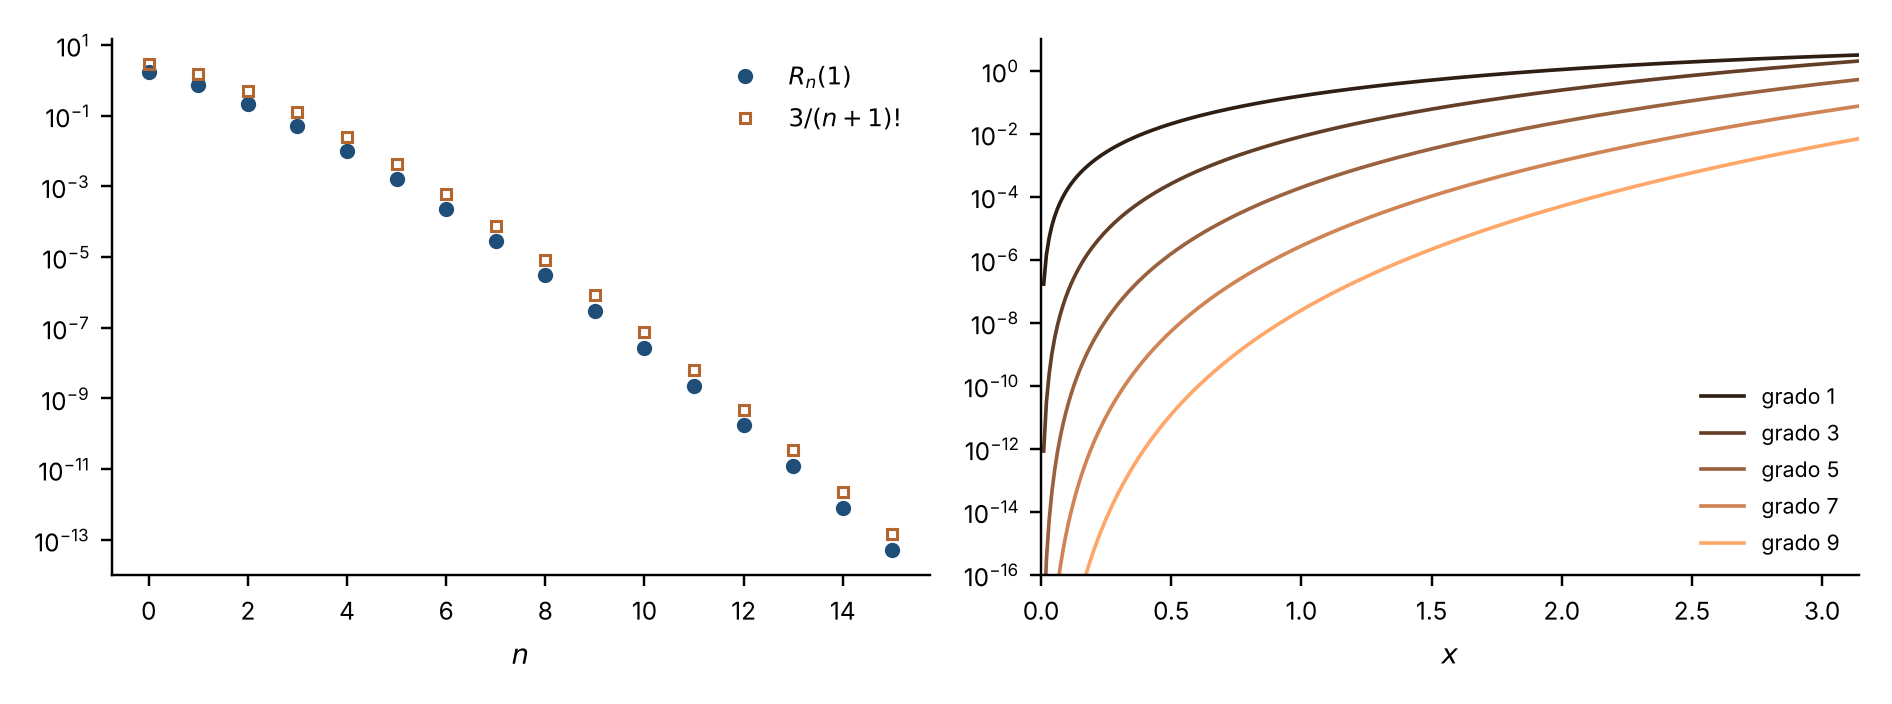
\includegraphics[width=\textwidth]{figure/errore_taylor.png}
\caption{A sinistra: l'errore $R_{n}(1)=e-\sum_{k=0}^{n}\frac1{k!}$ (punti blu) e la stima
$\frac3{(n+1)!}$ (punti rame), in scala logaritmica: la stima segue fedelmente l'errore vero.
A destra: l'errore $\abs{\sen x-T_{2n+1}(x)}$ in $[0,\pi]$ per $2n+1=1,3,5,7,9$; vicino a $0$ i
polinomi di grado alto sono straordinariamente precisi, mentre allontanandosi da $0$
l'errore cresce, pur restando sotto la stima $\frac{x^{2n+3}}{(2n+3)!}$ fornita dal resto di
Lagrange (\texttt{python/fig\_errore\_taylor.py}).}
\label{fig:errore-taylor}
\end{figure}

\begin{idea}[Come calcolano le calcolatrici]
Nessuna calcolatrice usa direttamente lo sviluppo di Taylor per $\sen x$ con $x$ grande:
la \cref{fig:errore-taylor} mostra che l'errore cresce rapidamente allontanandosi dal
centro. Si usa prima la periodicità e la simmetria per ricondurre l'argomento in un
intervallo piccolo, ad esempio $[0,\frac\pi4]$ (\emph{riduzione dell'argomento}), e poi un
polinomio di grado moderato, i cui coefficienti sono spesso leggermente modificati
rispetto a quelli di Taylor per distribuire l'errore uniformemente sull'intervallo
(polinomi di \emph{migliore approssimazione}). Un metodo diverso, che usa soltanto
somme e scorrimenti di cifre, è l'algoritmo CORDIC, ideato nel 1956 da Jack Volder alla
Convair per il calcolatore di navigazione del bombardiere B-58 e poi adottato nelle
prime calcolatrici tascabili.
\end{idea}

\subsection{L'irrazionalità del numero \texorpdfstring{$e$}{e}}

La stima \eqref{eq:stima-e} è così precisa da permettere di dimostrare che $e$ non è un
numero razionale. La dimostrazione, che risale a Fourier, è un piccolo gioiello: si
moltiplica la \eqref{eq:stima-e} per un fattoriale opportuno, in modo da rendere intero
tutto ciò che può esserlo, e si osserva che ciò che resta è un intero strettamente
compreso tra $0$ e $1$.

\begin{teorema}[Irrazionalità di $e$]\label{teo:e-irrazionale}
\index{numero di Nepero!irrazionalità}
Il numero $e$ è irrazionale.
\end{teorema}

\begin{schema}
\Ipotesi{la stima \eqref{eq:stima-e}: $0<e-\sum_{k=0}^{n}\frac1{k!}<\frac3{(n+1)!}$ per ogni $n\ge1$; \
$2<e<3$.}
\Tesi{non esistono interi $p,q\ge1$ con $e=\frac pq$.}
\end{schema}

\begin{strategia}
Ragioniamo per assurdo, supponendo $e=\frac pq$. Moltiplichiamo la \eqref{eq:stima-e}, con
$n=q$, per $q!$: il termine $q!\,e=p\,(q-1)!$ è intero, e lo è anche $q!\sum_{k=0}^{q}\frac1{k!}$, perché
ogni $k!$ con $k\le q$ divide $q!$. Allora anche $q!\,R_{q}(1)$ è un intero; ma la stima del resto
lo pone strettamente tra $0$ e $\frac3{q+1}$, che non supera $1$ se $q\ge2$. Un intero
strettamente compreso tra $0$ e $1$ non esiste.
\end{strategia}

\begin{dimostrazione}
Supponiamo per assurdo che sia $e=\frac pq$ con $p,q$ interi positivi. Poiché $2<e<3$, $e$ non è
intero, e quindi $q\ge2$. Applichiamo la \eqref{eq:stima-e} con $n=q$ e moltiplichiamo per
$q!$:
\[
  0<q!\,e-\sum_{k=0}^{q}\frac{q!}{k!}<\frac{3\,q!}{(q+1)!}=\frac3{q+1} .
\]
Il numero $q!\,e=q!\,\frac pq=p\,(q-1)!$ è intero; anche ogni $\frac{q!}{k!}=(k+1)(k+2)\cdots q$, con
$0\le k\le q$, è intero (per $k=q$ vale $1$). Dunque il numero
$N=q!\,e-\sum_{k=0}^{q}\frac{q!}{k!}$ è intero, e verifica $0<N<\frac3{q+1}\le1$, perché $q\ge2$. Ma non
esistono interi strettamente compresi tra $0$ e $1$: l'assurdo prova la tesi.
\end{dimostrazione}

\subsection{Approfondimento: una tavola dei logaritmi}
\label{subsec:tavola-logaritmi}

Il procedimento del paragrafo funziona male per il logaritmo, se si parte dallo sviluppo
di $\log(1+x)$: per $x=1$ la stima del \cref{sec:taylor-peano} dà soltanto
$\abs{R_{n}(1)}\le\frac1{n+1}$, e per avere $\log2$ con sei decimali esatti occorrerebbero milioni
di termini; per $x>1$, poi, i polinomi si allontanano dalla funzione. Giusti
\cite{giusti} suggerisce invece lo sviluppo di $\log\frac{1+x}{1-x}$, che si ottiene con lo stesso
artificio usato per l'arcotangente nella \cref{prop:sviluppo-arctg}.

\begin{proposizione}[Sviluppo di $\log\frac{1+x}{1-x}$]\label{prop:sviluppo-log-rapporto}
Per ogni intero $n\ge0$ e ogni $x\in(-1,1)$,
\begin{equation}\label{eq:sviluppo-log-rapporto}
\begin{gathered}
  \log\frac{1+x}{1-x}=2\Bigl(x+\frac{x^{3}}3+\frac{x^{5}}5+\dots+\frac{x^{2n+1}}{2n+1}\Bigr)+R(x),\\
  R(x)=2\int_{0}^{x}\frac{t^{2n+2}}{1-t^{2}}\,dt, \qquad
  \abs{R(x)}\le\frac{2\abs x^{2n+3}}{(2n+3)(1-x^{2})} ,
\end{gathered}
\end{equation}
e il resto $R(x)$ ha il segno di $x$.
\end{proposizione}

\begin{schema}
\Ipotesi{$n\ge0$ intero; \ $\abs x<1$.}
\Tesi{la \eqref{eq:sviluppo-log-rapporto}: il resto in forma integrale, la sua stima, e
$R(x)$ dello stesso segno di $x$.}
\end{schema}

\begin{strategia}
La derivata di $\log(1+x)-\log(1-x)$ è $\frac2{1-x^{2}}$, e $\frac1{1-t^{2}}$ è la somma della
progressione geometrica di ragione $t^{2}$, a meno di un resto esplicito. Integrando tra $0$
e $x$ la somma dà il polinomio, e nel resto il denominatore $1-t^{2}$ si minora con il suo
valore nell'estremo $x$.
\end{strategia}

\begin{dimostrazione}
Per $\abs t<1$, la formula della progressione geometrica (\cref{prop:geometrica}) con
ragione $t^{2}\neq1$ dà $\sum_{k=0}^{n}t^{2k}=\frac{1-t^{2n+2}}{1-t^{2}}$, cioè
\[
  \frac1{1-t^{2}}=\sum_{k=0}^{n}t^{2k}+\frac{t^{2n+2}}{1-t^{2}} .
\]
La funzione $g(x)=\log(1+x)-\log(1-x)=\log\frac{1+x}{1-x}$ è derivabile in $(-1,1)$, con
$g'(x)=\frac1{1+x}+\frac1{1-x}=\frac2{1-x^{2}}$ per la \eqref{eq:derivata-log} e la regola della catena,
e $g(0)=0$. Per la formula fondamentale (\cref{teo:formula-fondamentale}), integrando
l'uguaglianza precedente moltiplicata per $2$,
\[
  g(x)=2\int_{0}^{x}\frac{dt}{1-t^{2}}=2\sum_{k=0}^{n}\frac{x^{2k+1}}{2k+1}+R(x) .
\]
Sia $0<x<1$. Per $0\le t\le x$ si ha $1\ge1-t^{2}\ge1-x^{2}>0$, e quindi
$t^{2n+2}\le\frac{t^{2n+2}}{1-t^{2}}\le\frac{t^{2n+2}}{1-x^{2}}$; integrando tra $0$ e $x$, per il
confronto (\cref{teo:confronto-integrali}),
\[
  0<\frac{2x^{2n+3}}{2n+3}\le R(x)\le\frac{2x^{2n+3}}{(2n+3)(1-x^{2})} .
\]
Infine, poiché l'integrando è una funzione pari di $t$, la
sostituzione $t=-u$ mostra che $R(-x)=-R(x)$, e il caso $-1<x<0$ si riconduce al
precedente; per $x=0$ tutto è ovvio.
\end{dimostrazione}

La stima è tanto migliore quanto più $x$ è piccolo, e il quoziente $\frac{1+x}{1-x}$ assume
valori comodi se $x=\frac1{2N+1}$, con $N\in\N$: allora $\frac{1+x}{1-x}=\frac{2N+2}{2N}=\frac{N+1}N$ e
$1-x^{2}=\frac{4N(N+1)}{(2N+1)^{2}}$, sicché
\begin{equation}\label{eq:log-N}
\begin{gathered}
  \log\frac{N+1}N=2\sum_{k=0}^{n}\frac1{(2k+1)\,(2N+1)^{2k+1}}+R, \\
  0<R\le\frac1{2N(N+1)\,(2n+3)\,(2N+1)^{2n+1}} .
\end{gathered}
\end{equation}
Con $N=1$, cioè $x=\frac13$, si ottiene $\log2$: quattro termini ($n=3$) danno
\[
  \log2\simeq2\Bigl(\frac13+\frac1{81}+\frac1{1215}+\frac1{15\,309}\Bigr)=\frac{53\,056}{76\,545}=0{,}6931347\ldots ,
\]
con un errore positivo e inferiore a $\frac1{4\cdot9\cdot3^{7}}=\frac1{78\,732}<1{,}3\cdot10^{-5}$: dunque
$0{,}693134<\log2<0{,}693148$, e $\log2=0{,}6931\ldots$ con quattro decimali esatti; con lo
sviluppo di $\log(1+x)$, per garantire lo stesso errore, la stima richiederebbe quasi
ottantamila termini. Noto $\log2$, si calcolano
$\log3=\log2+\log\frac32$ (con $N=2$), $\log5=2\log2+\log\frac54$ (con $N=4$),
$\log7=\log2+\log3+\log\frac76$ (con $N=6$), e in generale il logaritmo di un primo $p$ dispari
da quelli dei primi minori, perché $p-1$ si scompone in essi, aggiungendo $\log\frac p{p-1}$
con $N=p-1$. Al crescere di $N$ la convergenza diventa sempre più rapida, e i
logaritmi dei primi successivi richiedono pochi termini. Per la proprietà $\log(ab)=\log a+\log b$, dai
logaritmi dei primi si ottengono per somma quelli di tutti gli interi, e dividendo per
$\log10=\log2+\log5$ i logaritmi decimali di Briggs, di cui parla la nota storica che
segue. Il programma costruisce questa piccola tavola con un errore garantito inferiore a
$10^{-13}$ per ciascun termine $\log\frac{N+1}N$, e la confronta con la libreria \texttt{math}.

\needspace{10\baselineskip}
\begin{python}[Una tavola dei logaritmi con errore garantito]
import math
from fractions import Fraction as F

def logN(N, tol=F(1, 10**13)):
    """log((N+1)/N) con x = 1/(2N+1), errore garantito < tol."""
    n = 0
    while F(1, 2*N*(N+1)*(2*n+3)*(2*N+1)**(2*n+1)) >= tol:
        n += 1
    x = F(1, 2*N + 1)
    T = 2 * sum(x**(2*k + 1) / (2*k + 1) for k in range(n + 1))
    return T, n + 1                  # valore e numero di termini

l2, t1 = logN(1)                     # log 2
l32, t2 = logN(2)                    # log 3/2
l54, t4 = logN(4)                    # log 5/4
l76, t6 = logN(6)                    # log 7/6
print("termini per N = 1, 2, 4, 6:", t1, t2, t4, t6)
tavola = {2: l2, 3: l2 + l32, 5: 2*l2 + l54}
tavola[7] = tavola[2] + tavola[3] + l76
for p, v in tavola.items():
    print(f"log {p} = {float(v):.12f}   (math.log: "
          f"{math.log(p):.12f})")
l10 = tavola[2] + tavola[5]
print(f"log10(2) = {float(tavola[2] / l10):.12f}")
\end{python}
\begin{risultato}
termini per N = 1, 2, 4, 6: 13 9 6 6
log 2 = 0.693147180560   (math.log: 0.693147180560)
log 3 = 1.098612288668   (math.log: 1.098612288668)
log 5 = 1.609437912434   (math.log: 1.609437912434)
log 7 = 1.945910149055   (math.log: 1.945910149055)
log10(2) = 0.301029995664
\end{risultato}

Per $N=1$ servono tredici termini, per $N=4$ e $N=6$ ne bastano sei. Gli errori dei
singoli termini si sommano, ma restano dell'ordine di $10^{-13}$: le dodici cifre decimali
stampate coincidono con quelle della libreria. Il valore $\log_{10}2=0{,}30103\ldots$ è quello
che si legge in ogni tavola dei logaritmi decimali.

\begin{notastorica}[Tavole e irrazionalità]
Le prime tavole dei logaritmi furono pubblicate da John Napier nel 1614 (\emph{Mirifici
logarithmorum canonis descriptio}); nel 1624 Henry Briggs pubblicò l'\emph{Arithmetica
logarithmica}, con i logaritmi decimali degli interi da $1$ a $20\,000$ e da $90\,000$ a
$100\,000$, calcolati con quattordici cifre. Quei calcoli, eseguiti a mano con metodi
ingegnosi ma faticosissimi, precedono di decenni la scoperta degli sviluppi in serie.
In seguito le serie fornirono i valori «di appoggio» con grande precisione, come
abbiamo fatto nel \S\ref{subsec:tavola-logaritmi}, mentre il
resto della tavola si completava per interpolazione con il metodo delle differenze
finite: così furono calcolate le grandi tavole francesi dirette da Gaspard de Prony
negli anni Novanta del Settecento, e lo stesso metodo ispirò la macchina alle differenze
di Charles Babbage. Le tavole furono lo strumento quotidiano di astronomi, navigatori e
ingegneri fino all'avvento delle calcolatrici elettroniche. L'irrazionalità
di $e$ fu dimostrata da Eulero nel 1737, mediante lo sviluppo in frazione continua; la
dimostrazione qui riportata, dovuta a Fourier, fu pubblicata nel 1815. Che $e$ sia
addirittura \emph{trascendente}, cioè non sia radice di alcun polinomio a coefficienti
interi, fu dimostrato da Charles Hermite nel 1873.
\end{notastorica}
